\chapter{Funciones generalizadas}

	
\begin{tikzpicture}
	\fill [left color=red!50, right color=teal!50] (0,0) rectangle (6.5,.1);
	\fill [left color=teal!50, right color=blue!50] (6.5,0) rectangle (11.5,.1);
	\end{tikzpicture}

\vspace{10mm}
\begin{adjustwidth}{50pt}{50pt}
\begin{ejemplo}
\vspace{2mm}

Hacemos un alto en el camino para ver el concepto fundamental en teoría de campos de \emph{función generalizada} y las derivadas funcionales en ese contexto.

Por ejemplo, si vemos algo así como $\ x\delta'(x)+(\sin x \ \delta(x^2-1) )'\, , \ $ ?`qué es la derivada de la delta de Dirac?. Entenderemos esto al finalizar este capítulo.

Además, una derivada funcional no es una función en sí, es una función generalizada, como la delta de Dirac (primer prototipo de función generalizada que aparece, pero no el único).
\vspace{2mm}

\end{ejemplo}
\end{adjustwidth}

\vspace{5mm}

\section{Función test}

\begin{definition}

Una función test $\  \boldsymbol{ u(x) } \ $es una función que cumple:	

\vspace{2mm} \hspace{1cm} $\bullet \qquad u(x) \in \mathcal C^\infty \, , \ $  es infinitamente derivable.

\vspace{2mm} \hspace{1cm} $\bullet \qquad \displaystyle \int_{-\infty}^{+\infty} u(x)\ \dd x \ < \ \infty\, , \ $ es finita.

\vspace{2mm} \hspace{1cm} $\bullet \qquad$ Tiene un \emph{soporte compacto}:

\vspace{2mm}\hspace{3cm} --- $u(x)=0 \quad \forall \ x \le a \ \wedge \ \forall \ x \ge b\ $ 

\vspace{2mm}\hspace{3cm} --- y conecta suavemente con $u(a)=u(b)=0$ (para que sea $ \mathcal C^\infty $)
\end{definition}

Un ejemplo típico de función test es $\qquad \displaystyle u(x) \ = \ \begin{cases}  \ e^{1/(x^2-1)} & \text{ si } \ -1<x<1 \\ \ 0 & \text{ resto} \end{cases}$

\begin{figure}[h]
    \begin{subfigure}{0.5\textwidth} %50% espacio reservado para img
	\centering
	\includegraphics[width=0.9\linewidth]{imagenes/img36-01.png} %img ocupará el 90% del sitio reservado
	\caption{Distinta de cero en $-1<x<1$}
	\label{fig:primer}
    \end{subfigure}
    \begin{subfigure}{0.5\textwidth}
	\centering
	\includegraphics[width=0.9\linewidth]{imagenes/img36-02.png}
	\caption{Conecta suave en $\pm 1$}
	\label{fig:segundo}
    \end{subfigure}
    \caption*{Ejemplo de función test}
    \label{fig:figura}
\end{figure}

Integración por partes: $\quad\displaystyle \int_{-\infty}^{+\infty} A'B\ \dd x \ = \ \eval{AB}_{-\infty}^{+\infty} \ - \ \int_{-\infty}^{+\infty} AB'\ \dd x$

Para la función test, $\ B=u(x)\, , \ $ como $\displaystyle \lim_{x\to \pm \infty} u(x) =0\, , $ tendremos que : 

\begin{equation}
\label{T36partes-test}	
 \displaystyle \boldsymbol{\int_{-\infty}^{+\infty}A'u \ \dd x \ = \ \int_{-\infty}^{+\infty} Au'\ \dd x }
\end{equation}




\vspace{10mm}
\section{Funciones generalizadas}

\begin{definition}

Una función generalizada a una función $f(x)$ 	asociada a una función test $u(x)$ es:

\begin{large}
\begin{equation}
\label{T36FG}
\boldsymbol{
f_u(x) \ = \ \int_{-\infty}^{+\infty} f(x)\ u(x)\ \dd x 
}	
\end{equation}
\end{large}
\end{definition}

Veamos las ventajas que tienen las funciones generalizadas.

\vspace{0.5cm}
\subsection{Derivada de una función generalizada}
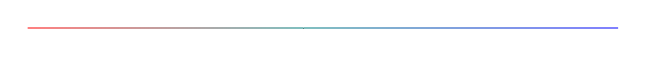
\begin{tikzpicture}
	\fill [left color=red!50, right color=teal!50] (0,0) rectangle (3.5,.01);
	\fill [left color=teal!50, right color=blue!50] (3.5,0) rectangle (7.5,.01);
	\end{tikzpicture}
\vspace{0.5cm}


$\boldsymbol{ f'(x)_u }= \displaystyle \int_{-\infty}^{+\infty} f'(x) \ u(x)\ \dd x 
\begin{matrix} \\ = \\ \text{\tiny{partes}} \end{matrix}
-\int_{-\infty}^{+\infty} f(x)\ u'(x)\ dd x = \int_{-\infty}^{+\infty} (-f(x))\ u'(x)\ \dd x = \boldsymbol{-f(x)_{u'}}$

Derivada segunda: llamo $g=f' \ \  \to \quad f''_u=g'_u=-g_{u'}=-f'_{u'}=-(-f)_{u''}=f_{u''}$

Derivada tercera $\quad f''_u=\cdots \ -f_{u'''}$

En general, 

\begin{equation}
\label{T36DFG}
\boldsymbol{
f^{n)}(x)_{\ u} \ = \ (-1)^n\ f(x)_{\ u^{n)}}
}	
\end{equation}

\vspace{5mm} La delta de Dirac es una función generalizada, veamos su derivada.

$\delta x = \displaystyle \int \delta(x) u(x) \dd x =u(0)$

$\left.
\begin{matrix}
\delta'(x) \displaystyle 
\begin{matrix} \\ = \\ \text{\tiny{def.}} \end{matrix}
\int \delta ' (x) \ u(x) \ \dd x
\begin{matrix} \\ = \\ \text{\tiny{partes}} \end{matrix}
-\int \delta(x) \ u'(x) \ \dd x =-u'(0) \qquad \
\\ \\
\delta'(x) \displaystyle
\begin{matrix} \\ = \\ \text{\tiny{prop.}} \end{matrix}
(-1)^1 \ \delta(x)_{\ u'} =-\delta(x)_{\ u'}
\begin{matrix} \\ = \\ \text{\tiny{def.}} \end{matrix}
-\int \delta x \ u' \ \dd x =-u'(0) \
\end{matrix}
\right\}
\  \boldsymbol{\delta'(x)=\displaystyle - \int \delta x \ u'(x)\ \dd x =-u'(0)}$

Ya tiene sentido derivar la función generalizada delta de Dirac.

\vspace{5mm}Nos preguntamos si se cumplirá la regla de Leibniz para las derivadas de funciones generalizadas:

$\triangleright \quad  (f(x)\ \delta(x))'_{\ u} \begin{matrix} \\ = \\ \text{\tiny{def.}} \end{matrix} \displaystyle \int (f(x)\ \delta(x))' \ u(x) \ \dd x \begin{matrix} \\ = \\ \text{\tiny{partes}} \end{matrix} \boldsymbol{ -\int f(x)\ \delta(x) \ u'(x)\ \dd x}$

$\triangleright \quad \displaystyle (f'(x)\ \delta(x)  + f(x)\ \delta'(x))_{\ u} = \int (f'(x)\ \delta(x)  + f(x)\ \delta'(x)) \ u(x) \ \dd x = \int f'(x)\ \delta(x)\ u(x)\ \dd x +\int f(x)\ \delta'(x)\ u(x)\ \dd x \begin{matrix} \\ = \\ \text{\tiny{partes int2}} \end{matrix} \int f'(x)\ \delta(x)\ u(x)\ \dd x -\int (f(x) \ u(x))'\ \delta(x)\ \dd x =\int f'(x)\ \delta(x) \ u(x)\ \dd x - \int (f'(x)u(x)+f(x)u'(x)) \dd x = \int \dd x \ \delta x \ (\cancel{f'(x)u(x)}-\cancel{f'(x)u(x)}-f(x)(u'(x)) = \boldsymbol{-\int \dd x \ \delta x \ f(x)\ u'(x)}$

\emph{Las funciones generalizadas cumplen la regla de derivación de Leibniz}.

\vspace{0.5cm}
\subsection{Composición de  funciones generalizadas}
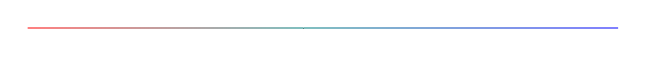
\begin{tikzpicture}
	\fill [left color=red!50, right color=teal!50] (0,0) rectangle (3.5,.01);
	\fill [left color=teal!50, right color=blue!50] (3.5,0) rectangle (7.5,.01);
	\end{tikzpicture}
\vspace{0.5cm}



\begin{definition}

Dadas $f(x)_{\ u}$ y $g(x)_{\ u}$, se define la composición de funciones generalizadas como:

$$\left ( f(g(x) \right)_{\ u} \ = \ \displaystyle \int f(g(x))\ u(x)\ \dd x$$	
\end{definition}

Hagamos un cambio de variable: $y=g(x) \leftrightarrow x=h(y)\; h=g^{-1}\, ; \quad \dd x=h'(y)\ \dd y\, . \ $ Para funciones de varias variables tendremos el jacobiano, $\ \dd x = |h'(y)| \ \dd y$

$f(g(x))_{\ u} = \displaystyle \int f(y)\ u(h)\ |h'(y)| \ \dd y $

Como $\ \begin{cases} \ y=g(x) \ \to \ \displaystyle \dv{y}{x}=g'(x) \\ \ x=h(y) \ \to \ \displaystyle \dv{x}{y}=h'(x) \end{cases} \ \displaystyle \dv{y}{x}=\dfrac 1{\dv{x}{y}} \ \to \ g'(x) =\dfrac 1{h'(y)} \ \leftrightarrow \ h'(y)=\dfrac 1{g'(x)}=\dfrac 1{g'(h)} $

$f(g(x))_{\ u} = \displaystyle \int f(x)\ u(h)\ \dfrac 1{|g'(h)|}\ \dd y$

De aquí obtendremos la fórmula más importante en TQC, por la frecuencia con que aparece.

\vspace{5mm} Hagamos que $\ f(x)=\delta x \ \text{ y } \ g(x)=f(x) \ $ y llamemos $\ h=g=f^-1$

$\delta (f(x))_{\ u} = \displaystyle \int \delta (y)\ u(g)\ \dfrac 1 {|f'(g)|}\ \dd y$

Tenemos el delta de Dirac de una función generalizada. La integral solo tomará valores distintos de cero cuando sea $y=0\quad $ \textcolor{gris}{$\ \left( \displaystyle \delta \Box \ ( \boxed{ \text{\textcolor{white}{xxx} }} ) = \boxed{ \Box=0} \ \right)$} 


$\delta (f(x))_{\ u} \ = \ \left[ \dfrac 1{|f'(g)|}\ u(g) \right]_{y=0}$

Si $y=f(x)=0$ supongamos que solo tiene una solución $x_0$. Como $x=g(y) \ \to x_0=g(0) \, , \  $ entonces

$\delta (f(x))_{\ u} \ = \ \left[ \dfrac 1{|f'(x_0)|}\ u(x_0) \right]_{y=0}$

Si hay dos soluciones para $y=f(x)=0 \ \to x_0, x_1$, como la integral es una suma, tendremos:

$\delta (f(x))_{\ u} \ = \  \dfrac {u(x_0)}{|f'(x_0)|} \ + \   \dfrac {u(x_1)}{|f'(x_1)|}$

Y así para todas la raíces de $f(x)=0$

$$\delta (f(x))_{\ u} \ = \ \displaystyle \sum_{i=0}^n  \dfrac {u(x_i)}{|f'(x_i)|} \, ; \quad x_i \  / \ f(x_i)=0 $$

Podemos escribir $\  u(x_i)=\displaystyle \int \delta(x-x_i) \ u(x)$ ya que,

$\begin{cases} \ t=x-x_0 \\ \ \dd t = \dd x \end{cases} \to \displaystyle u(x_i)=\int \delta(x-x_i) \ u(x) =\int \delta(t) \ u(t+x_i) \ \dd t = \eval{u(t+x_i)}_{t=0}=u(x_i)\, , \ $ así que,

$\delta (f(x))_{\ u} = \displaystyle \int \delta (y)\ u(g)\ \dfrac 1 {|f'(g)|}\ \dd y = \sum_{i=0}^n \dfrac 1 {|f'(x_i)|}\ \int \delta(x-x_i) \ u (x) \ \dd x$ 

La suma de integrales es la integral de la suma y, con ello, 

\begin{myblock}{Importante fórmula: delta de Dirac de una función generalizada}

\begin{large}
\begin{equation}
\label{T36TQCimpFmla}
\boldsymbol{
\delta(f(x))_{ \ u} \ = \ \displaystyle \int \sum_{i=0}^n \dfrac{\delta(x-x_i)}{|f'(x_i)|} \ u(x)\ \dd x	} \qquad \left( f(x_i)=0 \right)
\end{equation}
\end{large}
\end{myblock}

Normalmente, en los textos aparecerá esta fórmula de un modo esquemático como 

\begin{myalertblock}{Delta de Dirac de una función generalizada como aparece en los textos}
\begin{equation}
\label{T36TQCimpFmla-textos}	
\boldsymbol{
\delta(f(x)) \ = \ \displaystyle \sum_{i=0}^n \dfrac{\delta(x-x_i)}{|f'(x_i)|} 
} \qquad \qquad \left( f(x_i)=0 \right)
\end{equation}
\end{myalertblock}

pero la hemos de entender como una función generalizada aplicada a una integral con una función test.

$$\boldsymbol{ \left( \  \delta(f(x)) \ \right)_{\ u} \ = \ \displaystyle \left( \  \sum_{i=0}^n \dfrac{\delta(x-x_i)}{|f'(x_i)|} \ \right )_{\ u} }$$


\vspace{0.5cm}
\subsection{Ejemplos}
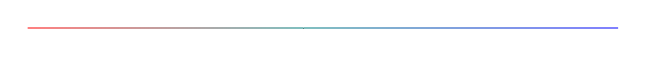
\begin{tikzpicture}
	\fill [left color=red!50, right color=teal!50] (0,0) rectangle (3.5,.01);
	\fill [left color=teal!50, right color=blue!50] (3.5,0) rectangle (7.5,.01);
	\end{tikzpicture}
\vspace{0.5cm}
\subsubsection{------ Ejemplo1}

Supongamos que al leer un libro de texto nos encontramos que nos dice que la siguiente integral tiene la solución trivial que se indica:
$\displaystyle \int \dd p \ p^2 \ \delta(E^2-p^2-m^2) \ = \ \sqrt{E^2-m^2} \, . \ $ Veamos como comprobarlo.

Comparando con la fórmula encontrada en el apartado anterior, $E^2-p^2-m^2=p$, ya qie es $p$ la variable ahora (por el $\dd p$). En nuestra fórmula aparece su derivada, $f'(p)=-2p$ y tenemos que encontrar los puntos $p_i \ / \ f(p_i)=0$, luego, $E^2-p^2-m^2= 0 \ \to \ p=\pm \sqrt{E^2-m^2}$, tomaremos $p_1$ con el signo $+$ y $p_2$ con el $-$, así,

$\delta(E^2-p^2-m^2)=\dfrac{\delta(p-p_1)}{|-2p_1|}+\dfrac{\delta(p-p_2)}{|-2p_2|}=\dfrac{\delta(p-p_1)}{2\sqrt{e^2-m^2}}+\dfrac{\delta(p-p_2)}{2\sqrt{e^2-m^2}}$

Y la integral, $\ \displaystyle I_1=\int \dd p \ p^2 \ \delta(E^2-p^2-m^2) \ = \int \dd p \ p^2 \ \left[ \dfrac{\delta(p-p_1)}{2\sqrt{E^2-m^2}}+\dfrac{\delta(p-p_2)}{2\sqrt{E^2-m^2}} \right] $

$I_1=\displaystyle \dfrac 1{\sqrt{E^2-m^2}}  \left[
\int \dd p \ p^2 \ \delta(p-p_1) \ + \ \dfrac 1{\sqrt{E^2-m^2}}\dd p \ p^2 \ \delta(p-p_2) \right]
\begin{matrix} \\ = \\ \text{\tiny{def.delta}} \end{matrix} 
\int \dfrac 1{2\sqrt{E^2-m^2}} \ (p_1^2+p_2^2)=\dfrac1{2\sqrt{E^2-m^2}} (E^2-m^2+E^2-m^2)= \dfrac {E^2-m^2}{\sqrt{E^2-m^2}}=\sqrt{E^2-m^2}$ \hspace{6cm} $\Box$



\begin{center}\rule{200pt}{0.2pt}\end{center}
\vspace{0.5cm}


La generalización de nuestra fórmula a varias dimensiones es:
$\ \ \boldsymbol{ \delta^{(d)}( \vec f( \vec x)) \ = \ \displaystyle \sum_i \dfrac {\delta^{(d)}( \vec x-  \vec x_i)}{|\text{J\tiny{acobiano} }( x_i))|}  }$

Veamos un nuevo ejemplo de dimensión-2:
\subsubsection{------ Ejemplo2}

Nuestro problema es calcular $\ \ \displaystyle I_2=  \int \dd x \int \dd y \ (x+y)\ \delta^{(2)} (\vec r-\vec R)\, , \ $ con $\vec r=(x,y)\ $ y $\ \vec R=(1+y,x^2-y^2)$

Ahora, $\vec f=\vec r-\vec R=(x,y)-(1+y,x^2-y^2)=(x-y-1,y-x^2+y^2)=(f_1,f_2)$

La matriz jacobiana, $\ J=\displaystyle \pdv{\vec f}{\vec x}= \mqty(  \displaystyle \pdv{f_1}{x} &  \displaystyle \pdv{f_1}{y} \\  \displaystyle \pdv{f_2}{x} &  \displaystyle \pdv{f_2}{y} )=\mqty(1&-1\\-2x&1+2y)$

El valor absoluto del determinante de la matriz jacobiana, es decir, el jacobiano en valor absoluto es: $|\det(J)|=|1+2y-2x|$

$f=0 \ \to \ \begin{cases}  \ f_1=0 \ \to \ x-1-y=0 \\  \ f_2=0 \ \to \ y-x^2+y¨2=0 \end{cases} x=1+y \ \to y-(1+y)^2+y^2=0 \ \to \ y=-1 \ \wedge \ x=0$

Los $x_i\ / \ f(x_i)=0 \ \leftrightarrow \ \ y=-1 \ \wedge \ x=0 \ \to \ (0,-1)$

El jacobiano, en $(0,.1) \ \text{ es } \ |1+2(-1)-2(0)|=|-1|=1$

Aplicando la fórmula, $\ \ \delta^{(2)} (\vec r-\vec R)  
\begin{matrix} \\ = \\ \text{\tiny{fórmua}} \end{matrix} 
\dfrac
{\delta(\vec r - (0,-1))}{1} \ $ y la integral del ejemplo 2 será

$I_2= \displaystyle \int \dd x \int \dd y \ (x+y) \ \delta(\vec r-(0,-1)) = \eval{(x+y)}_{(0,-1)}=0+(-1)=-1$

\vspace{5mm} Si hubiésemos tenido  $\ \displaystyle \int \dd x \int \dd y \ \delta(\vec r-\vec R)=\int \dd x \int \dd y \ \boldsymbol 1 \ \delta(\vec r-\vec R)=\eval{1}_{(0,-1)}=1$




\newpage
\begin{myexampleblock}{Función delta de Dirac}
	
	\begin{wrapfigure}{l}{0.4\textwidth} %izquierda- reservo 25% texto para img
    \centering
    \includegraphics[width=.95\linewidth]{imagenes/img36-03.png} %img ocupará 90% espacio rservado
    %\caption*{ }
    \label{T36fig-deltaD}
\end{wrapfigure}

La \emph{delta de Dirac} o  \emph{función delta de Dirac} es una función generalizada introducida por primera vez por el físico británico Paul Dirac.

$$ \delta_{a}(x)\equiv \delta (x-a)$$

siendo  $ \delta (x)\,$ la función que tiende a infinito cuando $x=0$ y, para cualquier otro valor de $x$, es igual a $0$.

\vspace{2mm} En física, la delta de Dirac puede representar la distribución de densidad de una masa unidad concentrada en un punto $a$. Esta función constituye una aproximación muy útil para funciones picudas y constituye el mismo tipo de abstracción matemática que una carga o masa puntual. 

\end{myexampleblock}


